\section{Theorie}
\label{sec:Theorie}
\subsection{Allgemeines zur Wärmepumpe}
Zu Betrachten sind zwei Wärmereservoirs mit verschiedener Temperatur.
Zwischen diesen findet Wärmeübertragung ohne äußere Einwirkung stets vom
wärmeren zum kälteren Wärmereservoir statt. Dies ist eine mögliche Formulierung des
zweiten Hauptsatzes der Thermodynamik oder kann alternativ in anderen Formulierungen
durch diese gezeigt werden. \newline
Eine Wärmepumpe ermöglicht durch Aufwendung mechanischer Energie den Transport von
thermischer Energie vom kälteren zum wärmeren Reservoir.
Eine Skizze zur Veranschaulichung der Funktionsweise einer Wärmepumpe ist in
Abbildung \ref{fig:waermepumpebild} zu sehen. Die Bezeichnungen in der Skizze werden
wie folgt umbenannt:
\begin{align}
p_\text{warm} &\coloneqq p_\text{b} & p_\text{kalt} &\coloneqq p_\text{a} \\
T_\text{warm} &\coloneqq T_1 & T_\text{kalt} &\coloneqq T_2
\end{align}

\begin{figure}
  \centering
  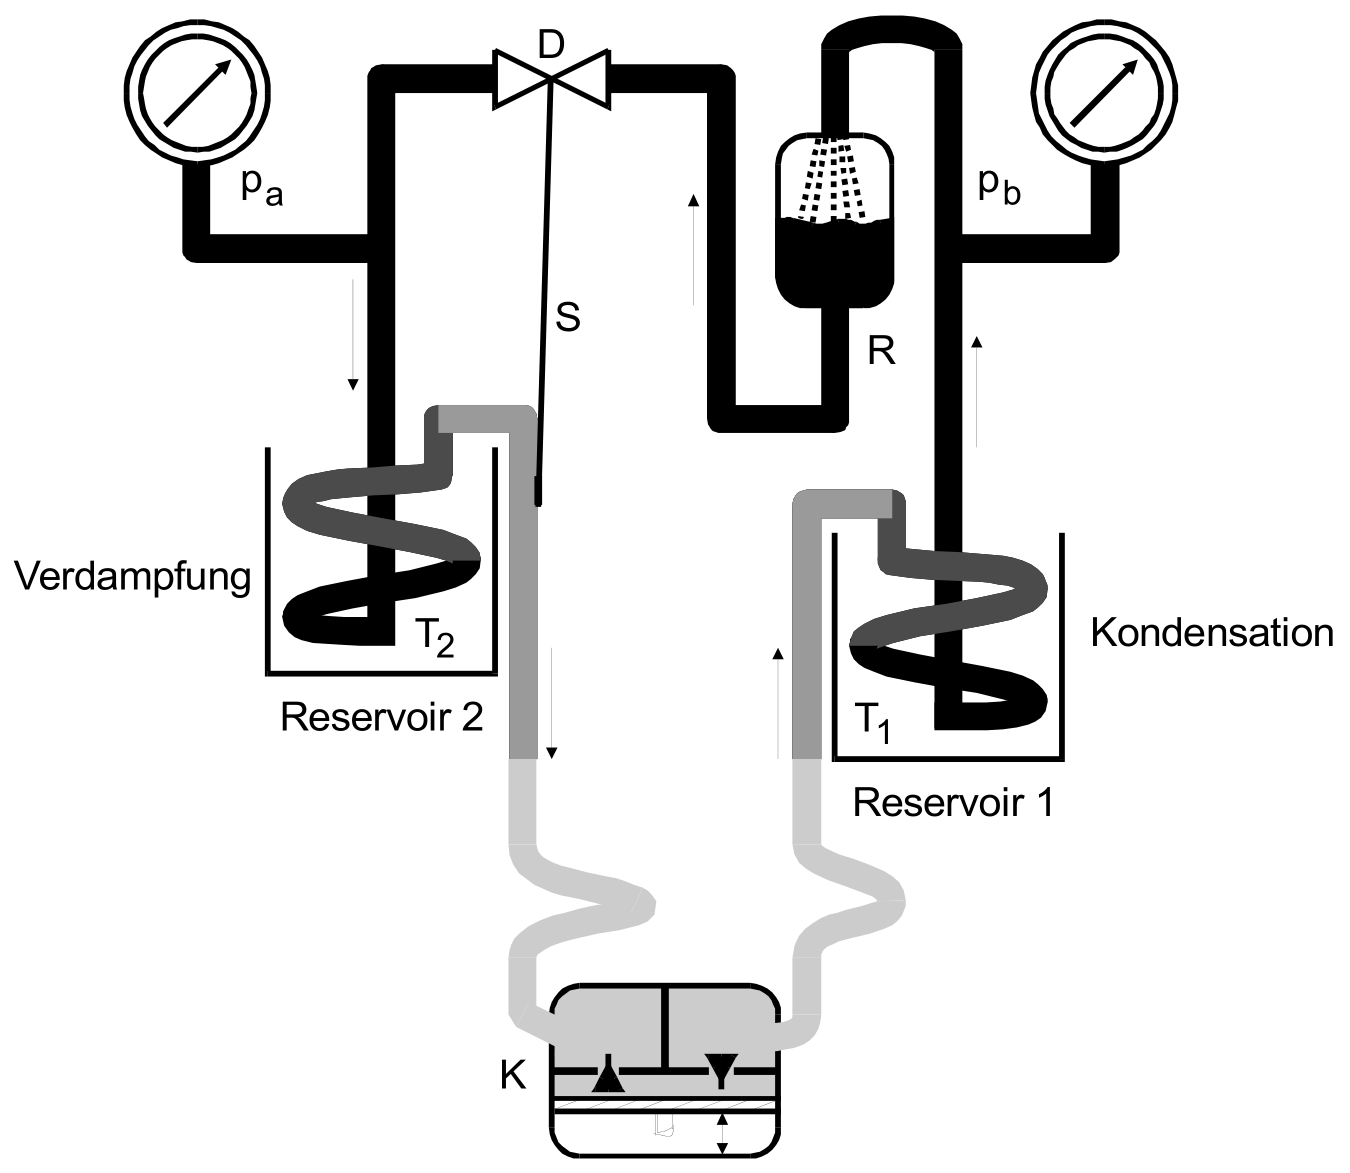
\includegraphics[width=300pt]{data/waermepumpe.png}
  \caption{Skizze einer Wärmepumpe, es gilt $p_\text{warm} > p_\text{kalt}$ und $T_\text{warm} > T_\text{kalt}$ \cite{Versuchsanleitung}}
  \label{fig:waermepumpebild}
\end{figure}

Ein reales Gas durchläuft die Wärmepumpe als Transportmedium. Dieses gibt beim Verdampfen
Wärme auf und gibt sie bei Verflüssigung wieder ab, sodass die transportierte Wärme
als Phasenumwandlungsenergie des verwendeten Gases vorliegt. Der Kompressor K ermöglicht
einen Kreislauf des Gases durch die Wärmepumpe. Das Gas ist bei der Temperatur $T_\text{warm}$
und dem Druck $p_\text{warm}$ flüssig und liegt bei der Temperatur $T_\text{kalt}$ und dem
Druck $p_\text{kalt}$ im gasförmigen Aggregatzustand vor. Reservoir 2 ist hier das
kältere Reservoir, welches Reservoir 2 wärmt. Das flüssige Gas durchströmt die Stelle D
und verdampft im Reservoir 2. Dabei wird dem dort befindlichen Stoff die Verdampfungswärme
$L$ pro Gramm entzogen. Daraufhin wird das Medium im Kompressor adiabatisch komprimiert,
sodass Temperatur und Druck steigen. In Reservoir 1 verflüssigt sich das Gas, indem es
die gleiche Wärmemenge, die es in Reservoir 2 aufgenommen hat, wieder abgibt.
Die restlichen Bestandteile der Apparatur und die Steuereinrichtungen D, S und R sind
ansonsten nicht weiter für die prinzipielle Funktionsweise der Wärmepumpe relevant.

\subsection{Die Güteziffer einer Wärmepumpe}
Wird der erste Hauptsatz der Thermodynamik auf das System einer Wärmepumpe angewandt,
so erhält man die Beziehung
\begin{equation}
  Q_\text{warm} = Q_\text{kalt} + A\,.
  \label{eqn:waermebilanz}
\end{equation}
Dabei ist $Q_\text{warm}$ die dem wärmeren Reservoir zugeführte Wärme,
$Q_\text{kalt}$ die dem kälteren Reservoir entnomenne Wärme und $A$ die aufgewandte
mechanische Arbeit.
Die Größe
\begin{equation}
  \nu = \frac{Q_\text{warm}}{A}
  \label{eqn:defnu}
\end{equation}
wird als Güteziffer der Wärmepumpe bezeichnet.
Erfolgt die Wärmeübertragung idealisiert vollständig reversibel, so gilt für die ideale
Güteziffer auch
\begin{equation}
  \nu_\text{id} = \frac{T_\text{warm}}{T_\text{warm} - T_\text{kalt}}\,.
  \label{eqn:nuid}
\end{equation}
Bei einer realen Wärmepumpe liegt ein irreversibler thermodynamischer Prozess vor,
sodass die reale Güteziffer $\nu_\text{real}$ stets echt kleiner als die ideale
Güteziffer ist.
